%% bare_conf.tex
%% V1.2
%% 2002/11/18
%% by Michael Shell
%% mshell@ece.gatech.edu

% setup page to suit conference specification using fancyhdr
\documentclass[conference,letterpaper]{IEEEtran}

%\usepackage{fancyhdr}
%\setlength{\paperwidth}{215.9mm}
%\setlength{\hoffset}{-9.7mm}
%\setlength{\oddsidemargin}{0mm}
%\setlength{\textwidth}{184.3mm}
%\setlength{\columnsep}{6.3mm}
%\setlength{\marginparsep}{0mm}
%\setlength{\marginparwidth}{0mm}
%
%\setlength{\paperheight}{279.4mm}
%\setlength{\voffset}{-7.4mm}
%\setlength{\topmargin}{0mm}
%\setlength{\headheight}{0mm}
%\setlength{\headsep}{0mm}
%\setlength{\topskip}{0mm}
%\setlength{\textheight}{235.2mm}
%\setlength{\footskip}{12.4mm}

%\setlength{\parindent}{1pc}

\usepackage{lipsum}

\usepackage{fancyhdr}

% some very useful LaTeX packages include:

\usepackage{cite}
\usepackage{url}
\usepackage{amsmath}
\usepackage{stfloats}
\usepackage[section]{placeins}

\usepackage{graphicx}
\usepackage{epstopdf}


%\usepackage{subfigure} % Written by Steven Douglas Cochran
                        % This package makes it easy to put subfigures
                        % in your figures. i.e., "figure 1a and 1b"
                        % Docs are in "Using Imported Graphics in LaTeX2e"
                        % by Keith Reckdahl which also documents the graphicx
                        % package (see above). subfigure.sty is already
                        % installed on most LaTeX systems. The latest version
                        % and documentation can be obtained at:
                        % http://www.ctan.org/tex-archive/macros/latex/contrib/supported/subfigure/


% Other popular packages for formatting tables and equations include:

%\usepackage{array}
% Frank Mittelbach's and David Carlisle's array.sty which improves the
% LaTeX2e array and tabular environments to provide better appearances and
% additional user controls. array.sty is already installed on most systems.
% The latest version and documentation can be obtained at:
% http://www.ctan.org/tex-archive/macros/latex/required/tools/

% Mark Wooding's extremely powerful MDW tools, especially mdwmath.sty and
% mdwtab.sty which are used to format equations and tables, respectively.
% The MDWtools set is already installed on most LaTeX systems. The lastest
% version and documentation is available at:
% http://www.ctan.org/tex-archive/macros/latex/contrib/supported/mdwtools/


% V1.6 of IEEEtran contains the IEEEeqnarray family of commands that can
% be used to generate multiline equations as well as matrices, tables, etc.


% Also of notable interest:

% Scott Pakin's eqparbox package for creating (automatically sized) equal
% width boxes. Available:
% http://www.ctan.org/tex-archive/macros/latex/contrib/supported/eqparbox/


% Notes on hyperref:
% IEEEtran.cls attempts to be compliant with the hyperref package, written
% by Heiko Oberdiek and Sebastian Rahtz, which provides hyperlinks within
% a document as well as an index for PDF files (produced via pdflatex).
% However, it is a tad difficult to properly interface LaTeX classes and
% packages with this (necessarily) complex and invasive package. It is
% recommended that hyperref not be used for work that is to be submitted
% to the IEEE. Users who wish to use hyperref *must* ensure that their
% hyperref version is 6.72u or later *and* IEEEtran.cls is version 1.6b
% or later. The latest version of hyperref can be obtained at:
%
% http://www.ctan.org/tex-archive/macros/latex/contrib/supported/hyperref/
%
% Also, be aware that cite.sty (as of version 3.9, 11/2001) and hyperref.sty
% (as of version 6.72t, 2002/07/25) do not work optimally together.
% To mediate the differences between these two packages, IEEEtran.cls, as
% of v1.6b, predefines a command that fools hyperref into thinking that
% the natbib package is being used - causing it not to modify the existing
% citation commands, and allowing cite.sty to operate as normal. However,
% as a result, citation numbers will not be hyperlinked. Another side effect
% of this approach is that the natbib.sty package will not properly load
% under IEEEtran.cls. However, current versions of natbib are not capable
% of compressing and sorting citation numbers in IEEE's style - so this
% should not be an issue. If, for some strange reason, the user wants to
% load natbib.sty under IEEEtran.cls, the following code must be placed
% before natbib.sty can be loaded:
%
% \makeatletter
% \let\NAT@parse\undefined
% \makeatother
%
% Hyperref should be loaded differently depending on whether pdflatex
% or traditional latex is being used:
%
\ifx\pdfoutput\undefined
\usepackage[hidelinks,hypertex]{hyperref}
\else
\usepackage[pdftex,hidelinks,hypertexnames=false]{hyperref}
\fi


\begin{document}
% paper title
\title{A Path Planning Method Based on Genetic Algorithms and Curve Fitting Techniques}
\newcommand{\Keywords}{Genertic Algorithms, Curve Fitting, Path Planning, Grid Method, Robotics}

% author names and affiliations
% use a multiple column layout for up to three different
% affiliations
\author{
\IEEEauthorblockN{Brock Kopp}
\IEEEauthorblockA{Mechatronics Engineering\\
	University of Waterloo\\
	Waterloo, Ontario\\
	brock.kopp@uwaterloo.ca}
\and
\IEEEauthorblockN{Karl Price}
\IEEEauthorblockA{Mechatronics Engineering\\
	University of Waterloo\\
	Waterloo, Ontario\\
	karldprice@gmail.com}
\and
\IEEEauthorblockN{Angelica Ruszkowski}
\IEEEauthorblockA{Mechatronics Engineering\\
	University of Waterloo\\
	Waterloo, Ontario\\
	aruszkow@uwaterloo.ca}}

% make the title area
\maketitle
\thispagestyle{plain}

% insert page header and footer here for IEEE PDF Compliant
\fancypagestyle{plain}{
\fancyhf{}	% clear all header and footer fields
\fancyfoot[L]{}
\fancyfoot[C]{}
\fancyfoot[R]{}
\renewcommand{\headrulewidth}{0pt}
\renewcommand{\footrulewidth}{0pt}
}

\pagestyle{fancy}{
\fancyhf{}
\fancyfoot[R]{}}
\renewcommand{\headrulewidth}{0pt}
\renewcommand{\footrulewidth}{0pt}


\begin{abstract}
% CRITERIA	(4 Senetences)
	% ?1. State the problem
	% ?2. Say why it�s an interesting problem
	% ?3. Say what your solution achieves
	% ?4. Say what follows from your solution
Navigation and path planning are critical components of developing robotic technology, where optimized path planning can improve efficiency and throughput of an industrial robotic manipulator. A genetic algorithm is used to plan a polynomial based trajectory which avoids collisions with any obstacles and minimizes trajectory path distance and dynamic constraints. The heuristic nature of the genetic algorithm allows it to determine a viable and efficient path for a manipulator quicky as it's environment changes. Algorithm results are verified by comparing with deterministic algorithms which produce the absolute best path.
\end{abstract}

\vspace{3mm}	%Brock

\begin{IEEEkeywords}
\Keywords
\end{IEEEkeywords}

\section{Introduction} \label{sec:introduction}
% CRITERIA	(1 Page)
	% 1.Describe the problem
	 % - Use Examples
	 % - Present the general case
	% 2.State your contributions
		% -Present a list of contributions
Path planning is a critical component of navigation technology, and a fundamental area in robotics research. Verifying path safety is critical for both the welfare of the robot as well as its surrounding environment, which can contain people or valuable infrastructure. The path must ultimately reach its destination while satisfying specified criteria, the most common of which is distance (or time). Another important criterion is path dynamics, where the forces and other dynamic characteristics of the robot are considered. Excessive acceleration and jerk cause stress on the robotic manipulator and degrade robot tracking characteristics, which are often a function of acceleration. These criteria are accounted for by relatively few common path planning algorithms \cite{elshamli04}.

Path planning techniques can be applied to industrial robotic manipulators to ensure efficient operation while maneuvering safely in the environment. Articulated manipulators are bounded to their configuration workspace, which is a two-dimensional representation of their allowable motion range \cite{kavraki96}. Frequently used algorithms for motion planning include probabilistic road maps, potential field methods, and neural network approaches \cite{sharir89,khosla88,rimon92,yang00}. Since every robot has a unique and complex task and environment, a robust solution is necessary. Genetic algorithms are especially suited for such complex optimization problems \cite{renner03}.

As a stochastic optimization technique, it is expected that a genetic algorithm will find the global optimum for a problem in a reasonable amount of time and computational cost. Due to the iterative evolutionary nature of genetic algorithms however, computational time may still be greater than other probabilistic algorithms. Overarching these concerns, the robustness of the genetic algorithm, combined with its ability to easily evaluate all path criteria of the optimization problem make it an appealing solution.

The robot's environment and obstacles will be represented in a discretized grid, and polynomial curve fitting techniques will be used to define the optimum path from the start to the end location through the specified environment. The curve fitting method helps simplify and expedite the generation of a desired path, compared to commonly used techniques such as rapidly exploring random trees \cite{rodriguez06}. The genetic algorithm will determine the polynomial coefficients which result in a curve with the greatest fitness, as determined by the constraints of the problem (namely path distance and jerk). A polynomial function was selected to describe the path since it inherently results in a continuous trajectory rather than traditional discontinuous way point based trajectories.

While there is no absolute best path planning algorithm for all situations, it is proposed that:

\begin{itemize}
	\item A Genetic Algorithm can effectively plan a path through a robotic manipulator's configuration space, producing a valid result 94\% of the time.
	\item The algorithm presented can plan a path which not only minimizes distance traveled, but also accounts for robotic manipulator dynamics such as acceleration and jerk.
	\item The algorithm can identify a viable solution which is within 1\% of the shortest distance as determined using a deterministic algorithm such as wavefront, while showing improvements to computation time.
\end{itemize}


\section{Background Review} \label{sec:background}
% CRITERIA	(1 page)
	% ?Materials & Method
	% ?Datasets
	% ?Materials (sources)
	% ?Methods (reference and brief description)
	% ?Proposed approach: algorithm
	% ?Equations and formulas

Path planning is an active area of research due to the complexity of the problem and the need for a robust solution applicable to various environments. Many algorithms exist, but none of the proposed algorithms are capable of encompassing all the problem constraints for various environments \cite{sariff06}.

Existing path planning solutions include reactive motion planning algorithms, graph and probabilistic based motion planning, and optimization based planning \cite{waslanderI}. Each of these has advantages and disadvantages with regards to planning a route through a robot's configuration space. Reactive planning algorithms such as potential field and wavefront methods are simple in concept however these are local approach methods and do not consider dynamic constraints. Some are inherently susceptible to local minima, making them unacceptable for obstacle avoidance \cite{koren91}. The wavefront method is designed to find the shortest path, and as such will be used as the benchmark against which results from the suggested algorithm will be measured. It is expected that while the suggested algorithm will generate a longer path, the dynamic constraints will be satisfied unlike in the wavefront solution.

Graph based planning offers a global approach. Graphs may be generated both deterministically (visibility graphs, cell decomposition, Voronoi diagrams), or randomly (probabilistic roadmaps). [10] Established algorithms (such as Dijkstra's shortest path search) are used to extract the shortest path from the graph \cite{dijkstra59}. However dynamics of the robot are ignored in the generation of the graph, and this is detrimental to the criterion of path smoothness. Challenges also arise when there are restrictive obstacles such as narrow passages, however research in areas such as probabilistic roadmaps (PRMs) offers promising solutions \cite{hsu03}. Optimization based planning offers more confidence in finding a global optimum, however it is hindered by a lack of robustness: a poorly formulated problem may not converge \cite{waslanderIII}. It is also difficult to define obstacles.

In an effort to provide a simple method of avoiding obstacles and defining a path, the manipulator's configuration space will be discretized using a grid-based approach, and curve fitting techniques will be employed to find the ideal path. Defining the environment with a grid-graph may not be the most effective (cell decomposition offers greater efficiency \cite{lingelbach04}), however it provides a simple way to defined obstacles as well as flexibility in representation. The grid will represent the configuration space for an articulated industrial robot. The grid cell size will define the computational resources required. A tradeoff between resolution in the grid and computational efficiency must be made.

To define the fitted curve, research has been done using B�zier curves \cite{choi10}. B�zier curves provide smooth paths that guarantee obstacle avoidance. While very effective for lower-dimensional problems, quartic or quintic functions begin to get very computationally expensive. That is why this paper aims to use curve fitting in combination with genetic algorithms to optimize the curve. The curve will be optimized by minimizing distance, maximizing smoothness (minimizing jerk), and ensuring a safe passage around all obstacles. Genetic algorithms are ideal for such complex optimization problems and offer good robustness as well \cite{zou12}.

The father of genetic algorithms, John Holland, modeled this machine intelligence technique after the evolution research by Darwin and the genetic ``survival of the fittest'' discovered in the natural, biological sphere. There are two natural learning epitomes available: the brain and evolution. Holland was inspired by the fact that the processes of natural evolution and natural genetics have become elucidated over decades of study in biology and molecular biology \cite{goldberg88}. The subtleties of the fundamental mechanisms of the brain, in contrast, are still shrouded in mystery. As such it seems clear to use the better understood model of genetic evolution as a platform for an optimization technique.

Research has already been done regarding the application of the parallel heuristic search method of genetic algorithms to curve fitting \cite{gulsen95,karr91,ismail08}. The goal is to find the coefficients that will define a path that with optimized path criteria. Thus each chromosome will contain a bitwise representation of each of the coefficient parameters.

Fitness will be determined based on distance as well as proximity to an obstacle. For safety, the robot should not approach too closely to an obstacle, thus the path must be planned to incorporate the robot dynamics such that obstacle avoidance will leave a sufficient safety margin. As such, smoothness is an implicit criterion.

The result will be a global path planning algorithm functional in a static environment. Dynamic environments are possible with the proposed algorithm, however computational efficiency must be optimized in order to minimize the time required to find the solution. This new applications offers a simple way to determine a path while taking into consideration all the path criteria.

\section{Method} \label{sec:method}
% CRITERIA	(2-3 pages)
	% -Check that each claim in the intro is addressed
	% -Forward reference evidence from a claim
	% -Present the experiments
	% -Analyze raw data
% OUTLINE
	% - Setup
		% - Criteria (Fitness)
			% - Distance (low weight since it doesn't really matter)
			% - Obstacle avoidance (Hight weight, mission critical)
			% - Minimize jerk (Mid weight)
		% - Touch breifly on encoding
			% - High order polynomial
			% - Chromozome - integer encoding
		% - Reporduction
			% - Random crossovers
		% - Mutation
			% - Defaults or Gusen's?
			% - Which worked out, why didn't the other?
		% - Initialization
			% - Random, pop size
		% - Termination
			% - Diversity convergence
			% - Or top half not coliding.
			% - Which worked out, why didn't the other?
	% - run with randomly generated environments (or at least
		% - 1-5 objects
		% - placed randomly w/o overlap
		% - varying but constrained size
		% - fized start/end points
		% - Run 1000 times
		% - analyze data
		% - store data (map and the resultant path)
%
The Genetic Algorithm (GA) was the subject of the experiments. Significant effort was expended setting up the GA in advance of testing, since without a well-structured algorithm, the testing was sure to show poor results. The GA was implemented in MATLAB, using the built-in GA libraries in order to avoid unnecessary development. While the base functionality was used, there remained many design considerations.

\subsection{Criteria and Fitness}
The aim of the implementation was to produce a path which minimized obstacle collisions, length and jerk of the path represented by a polynomial function. The fitness of an individual was based on an equation considering these three criteria.

In order to detect obstacle collisions, the algorithm iterated along the path, and checked at each point to see if the path was inside an obstacle. The chromosome was penalized proportionally to the number of path units within an obstacle. Collisions resulted in high punishments to the fitness value of an individual. It was important to divert the path around a collision point, as a single collision in the final solution would render that entire path invalid.

Length was calculated based on the integral line length formula. The weight of the line length was set to a medium penalty (relative to collisions and jerk). This was done since it is more important to find a valid solution that does not collide with any obstacles, than find the shortest path between the two points.

Finally, the maximum jerk value of the line was found by iterating the length of the fourth derivative of the path equation and recording the maximum value of this derivative. The jerk weight was set to make reduction in the jerk as important as reduction in the path length.

\subsection{Configuration Space}
Commanding a robotic manipulator's position is complicated by the fact that it cannot be specified as X-Y-Z coordinates, but rather must be commanded using joint angles. This is not intuitive for a human, and many existing planning techniques function using the more human-oriented X-Y or X-Y-Z coordinate systems, forcing the human to then convert their solutions to a joint space solution. As such, the robot's workspace was converted into a Configuration Space to allow the genetic algorithm to work with joint angles. Figure \ref{fig:ws2cs} shows both the workspace and the configuration space for a 2-DOF robot in an arbitrary workspace. The robotic manipulator's two degrees of freedom are denoted by the blue and red lines (each DOF respectively). The allowable robot configurations are represented in the Configuration Space by white areas, and collisions are represented by black.

\begin{figure}[h]
	\centering
	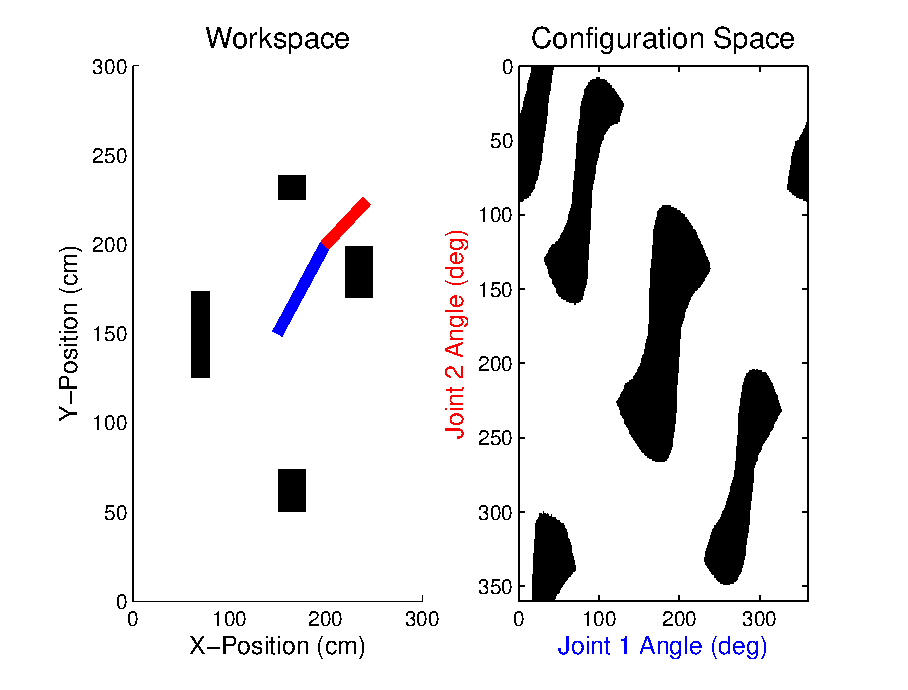
\includegraphics[width=\figWidth]{./figures/wp2cs.eps}
	\caption{Conversion from robot workspace to configuration space }
	\label{fig:ws2cs}
\end{figure}

In the configuration space, robot trajectories can be easily identified by either a human or a motion planning algorithm. This angle-angle plot can then be used to implement a polynomial trajectory, of which optimal coefficients can easily be solved using a Genetic Algorithm. The parameterized trajectory is denoted in Equation \ref{eq:polyTraj}.

\subsection{Population Initialization}

The population was randomly initialized with coefficient values in the range of -500 to 500. This range was imposed on the coefficients as it was found to provide a good compromise between promoting function variation while at the same time keeping it mitigated enough so that changes to coefficients each generation did not make too drastic a change to the shape of the path.

The population size was chosen to be 75, after research found that exiting solutions consistently used a population range of approximately 50-100 \cite{gulsen95}. This population number provides the necessary diversity in the population. Lower population values were found to converge to non-ideal solutions.

\subsection{Encoding}
The GA was developed using a linear encoding scheme, where a chromosome was defined to be an array of the polynomial function's coefficients (denoted as $\{P_0, \ldots, P_3\}$ in Equation \ref{eq:polyTraj}). Therefore, the GA would ultimately return the ideal set of coefficients for a function which would describe the optimal path for the robotic manipulator.

\subsection{Linear Constraints}
The path planning problem is a challenging optimization problem due to the various constraints involved. The goal is to generate a path that avoids all obstacles, as well as minimize the path length and minimize jerk. The problem is further constrained by the start and end points. The generated polynomial path must go through these desired start and end points.

To solve this constrained optimization problem, linear equality constraints are used. Linear equalities have the form:

\begin{equation}
A_{eq}x = b_{eq}
\end{equation}

Where x is a vector of the variables being optimized. For this project, the optimization variables are the coefficients of the polynomial.

For example, a second order polynomial $y = A + Bx + Cx^2$ through points $[2 , 4]$ and $[10 , 5]$ would have linear constraints of the form:
\begin{equation}
	\begin{bmatrix}
	1 & 10 & 10^2 \\
	1 & 2 & 2^2
	\end{bmatrix}
	\begin{bmatrix}
	A \\
	B \\
	C \\
	\end{bmatrix} =
	\begin{bmatrix}
	5 \\
	4 \\
	\end{bmatrix}
\end{equation}

\subsection{Selection}
A tournament selection method was used in this implementation to select chromosomes for cross-over. Two individuals were chosen for each tournament, allowing for an acceptable tradeoff between choosing a fit parent while promoting diversity in the offspring. This was one approach used to increase the diversity of the population when it was observed that the algorithm was getting stuck in invalid local minima.

\subsection{Reproduction and Mutation}
A heuristic reproduction method was used wherein the child is generated by taking the mean of the coefficients of the two parents, and then biased to resemble one of its parents. In this implementation, the child was biased 20\% towards the most fit parent using Formula \ref{crossoverEq}.

\begin{equation} \label{crossoverEq}
	child_i = parent_{i2} + 1.2 * (parent_{i1} - parent_{i2})
\end{equation}

As is common in non-binary encoded GA problems, the crossover method used in this implementation is based on a mean of the parents' genes. This is a key distinction from a traditional point crossover method, as it allows the genes to evolve from values that were not present in the initial population. If point crossover methods had been used, the best case scenario would simply involve the optimal configuration of coefficients from the initial, random population.

Mutation was achieved applying a random mutation to a coefficient within the individual selected to be mutated. In order to satisfy the linear constraints of the start and end points, if the function was rendered invalid by the mutation, a new random coefficient was chosen instead. The mutated coefficient must lie within the defined coefficient range of -500 to 500.

\subsection{Termination}
The termination criteria allow the GA to determine when it has reached the optimal solution to the problem. In this implementation, a termination criteria based on convergence of the fitness function was used. The mean fitness value over ten generations was averaged. When the averaged mean fitness value converged within 0.001 units, the algorithm was terminated. This is representative of a situation where the diversity of the function has been reduced, and the algorithm has converged on a minimum fitness value.

\subsection{Experiment} \label{sec:experiment}
In order to assess the performance of the GA approach, an extensive experiment was devised. The algorithm was run 600 times on 15 sets of randomly generated points in 3 environments (forming 45 different environments), with randomly positioned obstacles. Invalid combinations of point sets (such as a point which lies within an obstacle) were removed from the dataset and new points were randomly generated to replace them. The environments were chosen to represent environments which were sparsely populated with obstacles, through to dense population with obstacles. The results obtained by this experiment are presented Section \ref{sec:results}.

\section{Results} \label{sec:results}
-Stats \& Distributions

\section{Discussion} \label{sec:discussion}
% CRITERIA (Half a page)
	% - Main findigs
	% - What results mean
	% - Limitations of our method
	% - Comparison of our results (Campare to probabilistic path planning)
	% - Need for further studies
% OUTLINE - Main findings
	% - Worse distance than wavefront *complete (could use more info?)
	% - Expect success in reducing jerk *complete
		% - Find a metric
		% - Find a gold standard
	% - 100% success of finding a path w/o collisions
	% - Slower than wavefront *complete
	% - num generation *complete
%
Evaluating the performance of the genetic algorithm (GA) was complicated by its ability to consider many factors when determining the best path. These factors included path distance, vehicle dynamics and most importantly, obstacle avoidance. In order to determine a profile of the GA's performance, 600 independent tests were completed within 15 different environment configurations.

The length of the path generated by the GA approach was on average 0.7\% longer than the path generated by the wavefront method to which it was compared. The GA was able to determine a shorter path than the wavefront algorithm in 474 of 600 independent tests (79\%), while also minimizing manipulator jerk (sometimes at the cost of a longer path). The wavefront is a deterministic algorithm which will find a very short path around obstacles, with no consideration for vehicle dynamics. The GA works differently in that it is a stochastic algorithm that is sampling the environment in an effort to find the shortest path. As such, it can get stuck in a local minimum and not ultimately return the path of best possible fitness. While processes internal to the GA attempt to avoid these situations, it is not a perfect algorithm.

%% Speed
The GA was found to be significantly faster at finding a solution than the wavefront algorithm. The wavefront algorithm took an average of 17 minutes and 50 seconds to analyze the shortest path between two points in any of the three test spaces used in this study. In comparison, the genetic algorithm took an average of 5.15 seconds to find the optimal path, or roughly a 20700\% improvement.

While the absolute execution time of the algorithm (in seconds) is arbitrary and based on algorithm implementation, an improvement in execution time exceeding two orders of magnitude show a very conclusive improvement in performance over the wavefront algorithm. Both of these tests were performed using Matlab on a consumer grade desktop computer. With execution times in the seconds, it is possible that this algorithm could be implemented in real-time on a robotic manipulator whose environment was liable to change infrequently.

The algorithm was found to converge to a solution within an average of 12.3 generations, with a standard deviation of 2.58 generations. This represents a fast convergence of the algorithm to a single solution.

%% Collisions
It was expected to be able to develop an algorithm that would find a valid path which never collided with an obstacle. The results from the experiment show that the algorithm found a collision-free path 565 times in 600 (94\%) of the time. While this was not the anticipated result, it still constitutes a successful solution to the problem. In an industry application, if the algorithm produces a path which collides with an obstacle, it would simply re-initialize the population and start the evolution process again. With a run time of 5.15 seconds, restarting the algorithm would not be prohibitive for most applications.

%% Jerk
Since trajectories varied significantly between environments and start/end locations, a reference best-case scenario jerk could not be identified. The jerk of a path was therefore compared to another instance of the GA where jerk compensation was excluded from the fitness function. This allowed the effect of the jerk reduction to be quantified against a reference path, given a constant environment. It was found that the algorithm reduced the path's maximum jerk by an average of 192\%. Ultimately, the actual jerk of the robotic manipulator will be a function of the robot's speed, however by reducing path jerk, the robot can navigate its trajectory at a higher speed without exceeding allowable jerk.

\section{Conclusions} \label{sec:conclusions}
The results of path planning using genetic algorithms presented in this report show that genetic algorithms can effectively plan a path through a series of obstacles, and present an opportunity to improve on existing path planning techniques. By selecting the appropriate fitness criteria, it is possible to bias a genetic search algorithm to find a path which satisfies multiple geometric conditions. In this implementation, the path was optimized to have a short path length, no collisions and minimal jerk.

The algorithm is on average able to produce a path that is roughly the same length (100.7\%) as the shortest path as determined by the wavefront search method, while improving computation times by a factor of 100. 79\% of the time the algorithm finds a path that is shorter than that produced by the wavefront method, with much longer paths occurring occasionally (in the range of 0.1\% to 0.5\% of the time). Collision avoidance is of critical importance in the application of path planning to industrial manipulators. This implementation of genetic algorithms could produce a collision free path 94\% of the time. Finally, it was shown that the algorithm's jerk compensation was able to reduce path jerk by 11\%, when compared to the same algorithm without jerk compensation.

Through a transformation from Cartesian space to the manipulator's joint configuration space, a method has been suggested to apply these path planning techniques to obstacle avoidance for industrial manipulators.

A main limitation of this algorithm is that since it makes use of ordered pair polynomial functions, there is a limited geography through which it is possible to evolve (a single 'y' value per 'x' value). Invalid solutions would therefore be found by the algorithm in a situation where it necessary for the path to reverse upon itself to avoid an obstacle. This is a fundamental limitation of a polynomial. In order to overcome this limitation, a function family would need to be selected that could double back across the same x-axis location.

Future study should be considered to determine the optimal function order for varying degrees of environment complexity. Increasing function order will allow for a more complex path, but at the cost of increased complexity and computational requirements. Further expansion of this technique into three degree-of-freedom and greater manipulators will greatly improve upon the industrial applicability of this technique. Validation of realizable improvements to path dynamics is also necessary to validate the effectiveness of jerk and other dynamic compensation techniques.
\FloatBarrier

%	Figure Example
%--------------------------------------------------------------------------------%
% An example of a floating figure using the graphicx package.
% Note that \label must occur AFTER (or within) \caption.
% For figures, \caption should occur after the \includegraphics.
%
% \begin{figure}
% \centering
% \includegraphics[width=2.5in]{myfigure}
% where an .eps filename suffix will be assumed under latex,
% and a .pdf suffix will be assumed for pdflatex
% \caption{Simulation Results}
% \label{fig_sim}
% \end{figure}

%	Double Figure Example
%--------------------------------------------------------------------------------%
% An example of a double column floating figure using two subfigures.
% (The subfigure.sty package must be loaded for this to work.)
% The subfigure \label commands are set within each subfigure command, the
% \label for the overall fgure must come after \caption.
% \hfil must be used as a separator to get equal spacing
%
% \begin{figure*}
% \centerline{\subfigure[Case I]{\includegraphics[width=2.5in]{subfigcase1}
% where an .eps filename suffix will be assumed under latex,
% and a .pdf suffix will be assumed for pdflatex
% \label{fig_first_case}}
% \hfil
% \subfigure[Case II]{\includegraphics[width=2.5in]{subfigcase2}
% where an .eps filename suffix will be assumed under latex,
% and a .pdf suffix will be assumed for pdflatex
% \label{fig_second_case}}}
% \caption{Simulation results}
% \label{fig_sim}
% \end{figure*}

%	Table Example
%--------------------------------------------------------------------------------%
% An example of a floating table. Note that, for IEEE style tables, the
% \caption command should come BEFORE the table. Table text will default to
% \footnotesize as IEEE normally uses this smaller font for tables.
% The \label must come after \caption as always.
%
% \begin{table}
% increase table row spacing, adjust to taste
% \renewcommand{\arraystretch}{1.3}
% \caption{An Example of a Table}
% \label{table_example}
% \begin{center}
% Some packages, such as MDW tools, offer better commands for making tables
% than the plain LaTeX2e tabular which is used here.
% \begin{tabular}{|c||c|}
% \hline
% One & Two\\
% \hline
% Three & Four\\
% \hline
% \end{tabular}
% \end{center}
% \end{table}


% trigger a \newpage just before the given reference
% number - used to balance the columns on the last page
% adjust value as needed - may need to be readjusted if
% the document is modified later
% \IEEEtriggeratref{8}
% The "triggered" command can be changed if desired:
% \IEEEtriggercmd{\enlargethispage{-5in}}


\bibliographystyle{IEEEtran}
\bibliography{IEEEabrv,miGAplanning}

% that's all folks
\end{document} 